\documentclass[a4paper]{report}

% load packages
%\usepackage{showframe}
\usepackage[utf8]{inputenc}
\usepackage{enumitem}
\usepackage{listings}
\usepackage{courier}
\usepackage{hyperref}
\usepackage{graphicx}
\usepackage{float}
\usepackage[export]{adjustbox}

\setlength{\parskip}{1em}

\lstset{
  breaklines=true,
  basicstyle=\ttfamily,
  showstringspaces=false
}

\begin{document}

\title{Report of Programming Assignment 1 for CS 6301.001: Special Topics in Computer Science --- Introduction to Multi-Core Programming}

\author{Siming Liu}

\maketitle{}

\section*{Experiment Objective}
The experiment is intended to compare performance of three different kind of locks. There are Test-And-Set (aka TAS), Test-Test-And-Set (aka TTAS) and Tournament lock.

\section*{Experiment Method}
For each lock ($l$), I launch multiple threads ($n$) to increase a shared variable concurrently.
In each thread, it loops multiple times ($c$).
These threads use one single lock to enter and leave critical section. In the thread running function, there are just simply calling \lstinline{Lock()}, adding shared variable by one and calling \lstinline{Unlock()} and looping them by $c$ times.
A high accurate timer is used to calculate the total time from starting of these threads to end of these threads.
I call the procedure above a test unit for $l$ lock, $n$ threads and $c$ loop times, denoted by $tu(l, n, c)$.
The result of a test unit is total running time of these threads in nanoseconds.
In order to avoid outliers, I do a test unit for several times $r$ and then get an average time, denoted by $t = atu(l, n, c, r)$.

In order to fully evaluate performance, I change the number of threads from $1$ to the number of logical cores ($m$) in the machine and then get several pair values, denoted by $(n_1, t_1), (n_2, t_2), \ldots, (n_m, t_m), t_i = atu(l, n_i, c, r)$. Thus I get a line for lock $l$ by putting these pair values in the coordinate ($x$ axis: $n$, $y$ axis: $t$ nanoseconds) and linking these points together.

There are totally three locks.
For each lock, I test and get a line and combine them in a plot.
So from the plot, we could compare performance of three locks clearly.

\section*{How to Implement}
I use \lstinline{C++} and several \lstinline{C++11} features to implement it.
The program called \lstinline{lock_compare} could receive three parameters: $n$, $c$ and $r$.

Basically, for each lock, I implement a class and expose two public functions \lstinline{Lock} and \lstinline{Unlock}.
For example, \lstinline{class TASLock} for TAS, \lstinline{class TTASLock} for TTAS.
Because Tournament lock uses a binary tree structure in which each node is a Peterson lock, there are two classes for implementing it: \lstinline{class PetersonLock} and \lstinline{class TournamentLock}.
For Tournament class, the current level is $4$.
It is hard-coded in the source code by \lstinline{static constexpr std::size_t level_ = 4;}.
In order to achieve mutual exclusion, I use \lstinline{C++11}'s \href{http://en.cppreference.com/w/cpp/atomic}{Atomic Operations Library} for the types of the internal variables in each lock class.

In terms of testing, I implement a base class called \lstinline{class BaseTester} filled with common logic for all tester.
And nearly for each lock, there is a tester class that is inherited from \lstinline{class BaseTester}.
In the end, there is a \lstinline{class Tester} as a only one entry for testing.
It does all necessary tests by calling each tester and output result points.
I also write a \lstinline{R} script to generate a plot by using the output of testing program.

\section*{How to Verify Mutual Exclusion}
It is simple.
After each unit test $tu(l, n, c)$, the shared variable should be equal to $n \cdot c$.
So checking this value after each unit test, if the condition is violated, I throw an exception and catch it in the top level to stop testing procedure because mutual exclusion is violated.

\section*{Testing Environment and Experiment Results}
Tests are done in the platform called \href{https://www.tacc.utexas.edu/}{TACC}.
It is a distributed supercomputer clusters.
I use one of visualization node to do the test.
A visualization node have 2 Intel Xeon E5-2680 processors (16 total cores) and 32GB of memory.
Command \lstinline{lock_compare 16 1000000 16} are used to launch testing.

The plot below is the test result.
We could clear see that the performance of three locks from slow to fast is Tournament, TAS, TTAS.

\begin{figure}[H]
  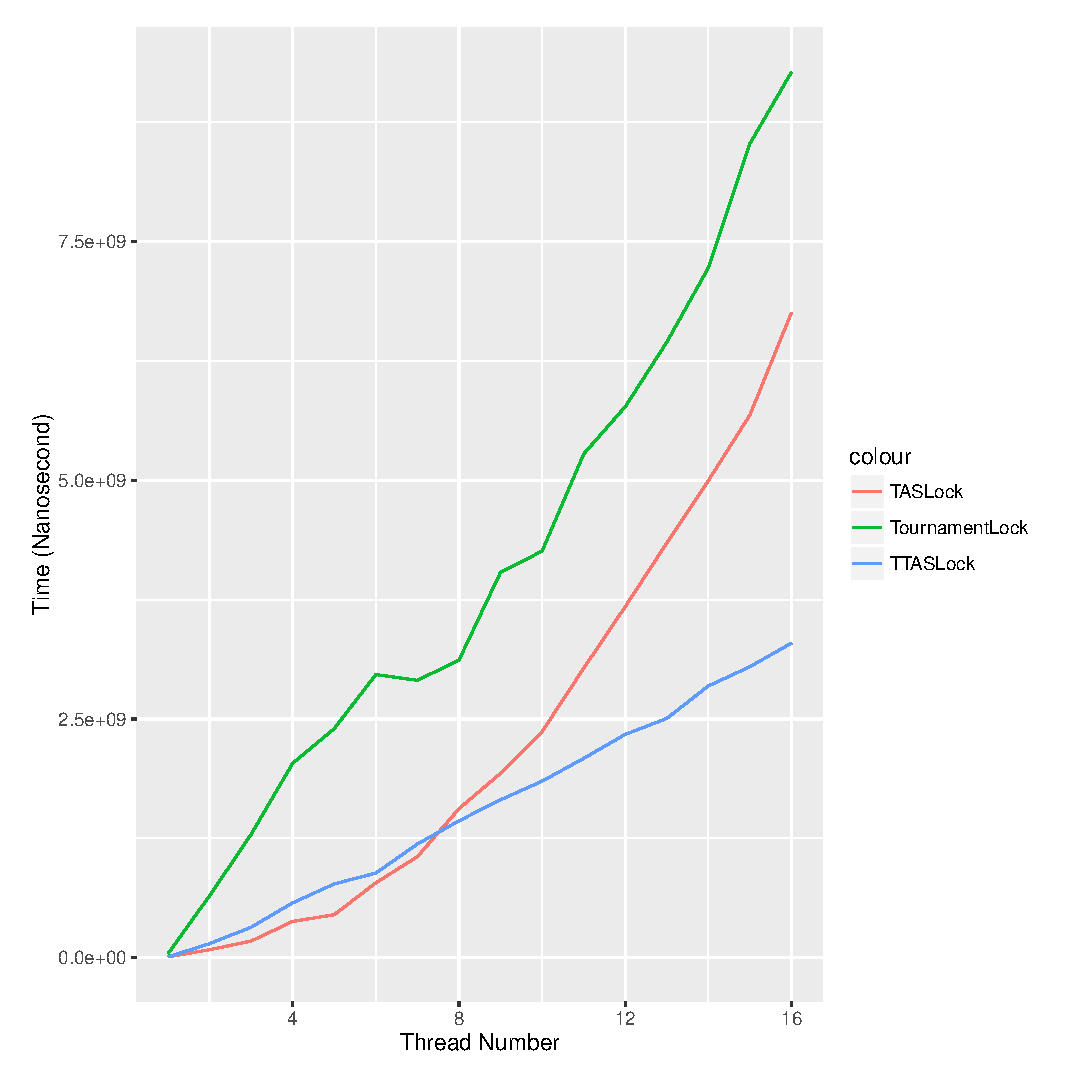
\includegraphics[scale=0.8]{result-tacc-7637283}
  \caption{Test Result on TACC}
\end{figure}

\end{document}
